\documentclass{article}

% if you need to pass options to natbib, use, e.g.:
%     \PassOptionsToPackage{numbers, compress}{natbib}
% before loading neurips_2024


% ready for submission
% \usepackage{neurips_2024}

\usepackage[preprint]{neurips_2024}
\usepackage[margin=0.65in]{geometry}

% to compile a preprint version, e.g., for submission to arXiv, add add the
% [preprint] option:
%     \usepackage[preprint]{neurips_2024}


% to compile a camera-ready version, add the [final] option, e.g.:
%     \usepackage[final]{neurips_2024}


% to avoid loading the natbib package, add option nonatbib:
%    \usepackage[nonatbib]{neurips_2024}


\usepackage[utf8]{inputenc} % allow utf-8 input
\usepackage[T1]{fontenc}    % use 8-bit T1 fonts
\usepackage{hyperref}       % hyperlinks
\usepackage{url}            % simple URL typesetting
\usepackage{booktabs}       % professional-quality tables
\usepackage{amsfonts}       % blackboard math symbols
\usepackage{nicefrac}       % compact symbols for 1/2, etc.
\usepackage{microtype}      % microtypography
\usepackage{xcolor}         % colors
\usepackage{amsmath}
\usepackage{graphicx}



\title{Directed vs. Undirected Graphical Models for Uncertainty-Aware Heart Disease Diagnosis}


% The \author macro works with any number of authors. There are two commands
% used to separate the names and addresses of multiple authors: \And and \AND.
%
% Using \And between authors leaves it to LaTeX to determine where to break the
% lines. Using \AND forces a line break at that point. So, if LaTeX puts 3 of 4
% authors names on the first line, and the last on the second line, try using
% \AND instead of \And before the third author name.


\author{
  Chan Cheah Cha \\
  A0189006A \\
  \And
  Li Zongzhao \\
  A0318503L \\
  \And
  Nguyen Thuan Hung \\
  A0219727W \\
  \And
  Wang Zhiyang \\
  A0318102W \\
  \And
  Wang Yi \\
  A0314485B \\
}


\begin{document}

\maketitle

\begin{abstract}
    We compare Bayesian Networks and Markov Random Fields for uncertainty-aware heart disease diagnosis on the UCI Cleveland dataset (303 patients, 13 features). Both the structure-learned BN and tuned MRF achieve AUC\,=\,0.916, matching discriminative baselines; parameterization quality (BDeu priors, MI reweighting) drives a +0.10 AUC gain exceeding any directed-vs-undirected gap. MCMC Gibbs sampling validates against exact inference and quantifies diagnostic test value via predictive entropy. GMMs complement the pipeline with EM imputation and unsupervised phenotyping.
\end{abstract}

\section{Introduction}
  Reliable heart disease diagnosis requires models that not only predict
  outcomes but also quantify uncertainty under incomplete clinical evidence.
  This project evaluates the comparative strengths of Directed Graphical
  Models (Bayesian Networks) and Undirected Graphical Models (Markov Random
  Fields). In this report, we explore the trade-offs between
  three paradigms in Probabilistic Graphical Models (PGMs):
  \begin{enumerate}
      \item \textbf{Bayesian Networks (BNs):} Representing causal hierarchies
            (Risk Factors $\rightarrow$ Disease $\rightarrow$ Symptoms), with
            exact inference via Variable Elimination and parameter learning
            under both MLE and BDeu priors.
      \item \textbf{Markov Random Fields (MRFs):} Representing symmetric
            correlations via MI-reweighted pairwise potentials, with Belief
            Propagation inference.
      \item \textbf{Gaussian Mixture Models (GMMs):} EM-based unsupervised
            clustering and generative classification on continuous features,
            serving as a latent-variable baseline.
  \end{enumerate}
  We benchmark these against four discriminative baselines (Logistic
  Regression, Naive Bayes, Random Forest, SVM) using a unified 5-fold
  stratified cross-validation framework covering nine metrics, and extend
  the analysis with calibration assessment, robustness experiments under
  missing evidence, failure-mode analysis, feature importance rankings,
  clinical threshold optimization, and MCMC-based latent variable inference.


\section{Problem Statement}

  Given patient attributes such as age, cholesterol levels, blood pressure,
  and symptoms (e.g.\ chest pain, ECG abnormalities), how can we estimate
  the posterior probability of heart disease while properly quantifying
  uncertainty? By representing a set of patient attributes
  $\mathbf{X} = \{x_1, x_2, \dots, x_n\}$, our goal is to estimate the
  posterior probability $P(Y{=}1 \mid \mathbf{X}_{\text{obs}})$ where $Y$ is
  the presence of heart disease and
  $\mathbf{X}_{\text{obs}} \subseteq \mathbf{X}$ is a (possibly incomplete)
  subset of observed features. We specifically address:
\begin{itemize}
      \item How does the choice of directed vs.\ undirected edges affect
            robustness and uncertainty calibration when key diagnostic
            features (e.g.\ \texttt{ca}, \texttt{thal}) are unavailable?
      \item Can post-hoc calibration (Platt scaling) close the calibration
            gap between graphical models and discriminative baselines?
      \item How does MCMC approximate inference (Gibbs sampling) compare
            to exact inference when clinical variables are structurally
            latent?
  \end{itemize}


\section{Related Work}

Bayesian Networks have a long history in clinical decision support.
\citet{korb2011bayesian} survey their use for encoding expert knowledge as
directed acyclic graphs, while \citet{koller2009pgm} provide the theoretical
foundations for structure learning, parameter estimation, and exact inference
that underpin the BN variants in this study. Undirected models (MRFs) offer
an alternative when the causal direction between variables is ambiguous:
pairwise potentials capture symmetric symptom correlations without requiring a
DAG~\cite{murphy2012mlpp}. Despite extensive individual use, direct empirical
comparisons of BNs and MRFs on the \emph{same} clinical dataset---with matched
evaluation protocols covering discrimination, calibration, and robustness
under missing evidence---remain scarce.

On the probabilistic side, calibration has emerged as a critical yet
under-reported quality dimension for medical AI. \citet{naeini2015ece}
introduced Expected Calibration Error (ECE) and showed that many classifiers
with high AUC still produce unreliable probability estimates;
\citet{platt1999scaling} proposed post-hoc sigmoid recalibration (Platt
scaling) to address this gap. Our work bridges these threads by evaluating
both discrimination \emph{and} calibration across directed, undirected, and
discriminative models, and further extends the analysis with MCMC-based
latent variable inference and EM-driven unsupervised phenotyping.


\section{Methodology}

\subsection{Data Cleaning and Preprocessing}

The UCI Heart Disease dataset (\url{https://www.archive.ics.uci.edu/dataset/45/heart+disease}) serves as our benchmark for evaluating probabilistic graphical models. It includes structured clinical features such as age, cholesterol, resting blood pressure, and heart rate. The dataset consists of 303 patient records with 13 clinical features and a target variable, \texttt{num}, representing the presence of heart disease on a scale of 0 (healthy) to 4 (severe). For this study, we treat the problem as a binary classification task where \texttt{num} $> 0$ indicates a positive diagnosis.


Exploratory analysis revealed a high level of data integrity, with missing values present in only two features: \texttt{ca} (4 missing) and \texttt{thal} (2 missing). Given that these represent less than 2\% of the total instances, we applied \textbf{mode imputation} to maintain the sample size without introducing significant bias.

\subsubsection{Feature Analysis and Selection}
Correlation analysis against \texttt{num} (Figure~\ref{fig:feature_correlation}) identified the strongest positive predictors: fluoroscopy vessel count (\texttt{ca}, $r\!=\!0.52$), thallium stress test (\texttt{thal}, $r\!=\!0.51$), and exercise ST depression (\texttt{oldpeak}, $r\!=\!0.50$). Maximum heart rate (\texttt{thalach}, $r\!=\!{-}0.42$) showed the strongest inverse relationship. As shown in Figure~\ref{fig:pairplot}, the diagonal KDE plots reveal sharp peaks for healthy patients near zero in \texttt{oldpeak} and \texttt{ca}, while scatter plots identify ``danger zones'' (e.g., \texttt{oldpeak}\,$>2.0$ and \texttt{thalach}\,$<120$).

These directional relationships (e.g., age$\rightarrow$outcomes) justify a causal BN, while the strong symmetric correlations between symptoms (e.g., \texttt{thalach} and \texttt{oldpeak}) motivate an MRF as a complementary model.


\subsection{Bayesian Network (Directed)}

We construct a 3-layer Bayesian Network to represent the causal dependencies between clinical risk factors, the underlying heart disease state, and the observable symptoms. Our structure follows a directed acyclic path:
\begin{equation}
    \text{Risk Factors} \rightarrow \text{Heart Disease} \rightarrow \text{Symptoms}
\end{equation}

\begin{enumerate}
\item \textbf{Layer 1 (Risk Factors):} \texttt{age}, \texttt{sex}, \texttt{fbs}, \texttt{chol}, \texttt{trestbps}
\item \textbf{Layer 2 (Disease Status):} \texttt{num} (the target variable)
\item \textbf{Layer 3 (Symptoms/Indicators):} \texttt{cp}, \texttt{thalach}, \texttt{exang}, \texttt{oldpeak}, \texttt{slope}, \texttt{ca}, \texttt{thal}, \texttt{restecg}
\end{enumerate}

We followed an iterative improvement process to optimize model performance and robustness:
\begin{itemize}
    \item \textbf{Addressing Data Sparsity (BDeu Prior):} Our initial Maximum Likelihood Estimation (MLE) suffered from "zero-count collapse," where sparse data caused the model to assign zero probability to valid clinical scenarios. By transitioning to \textbf{BDeu prior estimation}, which regularizes the CPTs using virtual pseudo-counts, we ensured the model remains robust in sparse regimes.
    \item \textbf{Enriching the Topology:} In Figure \ref{fig:enhanced_bayesian}, by introducing direct edges (e.g., \texttt{age} $\rightarrow$ \texttt{thalach}), we captured physiological dependencies that exist independently of the binary disease state, improving model calibration.
    \item \textbf{Automated Structure Learning:} In Figure \ref{fig:bayesian_hc}, using \textbf{Hill-Climbing search}, we moved beyond fixed domain knowledge to discover data-driven dependencies, which provided the most significant performance gain.
\end{itemize}


To quantify the impact of our architectural refinements, we compared several variants of our Bayesian Network against standard machine learning baselines. As summarized in Table \ref{tab:bn_improvements}, the transition from a manually defined topology to a data-driven structure via Hill-Climbing, combined with Bayesian regularization, consistently closed the performance gap.


\subsubsection{Parameter Learning}
We estimated CPDs using Maximum Likelihood Estimation (MLE), revealing clear clinical discriminators (e.g., \texttt{exang} probability rises from 14\% to 55\% with disease; \texttt{cp=3} yields $P(\text{num}=1)=0.755$). However, MLE suffered from zero-count collapse in sparse CPT cells (72 parent combinations with many unobserved). Applying \textbf{BDeu prior estimation} regularizes the CPDs with virtual pseudo-counts, ensuring numerically stable inference. We evaluate all BN variants against discriminative baselines in Section~4.

\subsubsection{Limitations}
The DAG remains sensitive to discretization loss. Future work could incorporate continuous modeling extensions (e.g. Gaussian BNs) to preserve precision and mitigate sample-size sparsity.

\subsection{Markov Random Field (Undirected)}

We construct an undirected Markov Random Field (MRF) to represent the joint probability distribution and symmetric correlations among clinical risk factors, the underlying heart disease state, and the observable symptoms. Our structure mirrors a 3-layer architecture, but with undirected edges parameterized by unary and pairwise potentials:
\begin{equation}
    \text{Risk Factors} \longleftrightarrow \text{Heart Disease} \longleftrightarrow \text{Symptoms}
\end{equation}

\begin{enumerate}
\item \textbf{Layer 1 (Risk Factors):} \texttt{age}, \texttt{sex}, \texttt{fbs}, \texttt{chol}, \texttt{trestbps}
\item \textbf{Layer 2 (Disease Status):} \texttt{num} (the target variable)
\item \textbf{Layer 3 (Symptoms/Indicators):} \texttt{cp}, \texttt{thalach}, \texttt{exang}, \texttt{oldpeak}, \texttt{slope}, \texttt{ca}, \texttt{thal}, \texttt{restecg}
\end{enumerate}

We followed an iterative improvement process to optimize model performance and robustness:
\begin{itemize}
    \item \textbf{Factor Regularization (Laplace Smoothing):} To address data sparsity and prevent zero-probability assignments, we applied \textbf{Laplace Smoothing ($\alpha$)} during empirical potential initialization. The mechanism and necessity of this regularization step are identical to the BDeu prior estimation discussed previously in the directed network section.
    \item \textbf{Interaction Reweighting (Mutual Information):} Rather than treating all pairwise dependencies equally, we enriched the factor learning process by incorporating \textbf{Mutual Information (MI) reweighting} ($\gamma > 0$). This dynamically adjusted the potential strengths $\phi(x) = \phi_{base}(x)^{1 + \gamma \cdot W_{MI}}$ according to their true pairwise dependency, prioritizing paths with better signal-to-noise ratios.
    \item \textbf{Hyperparameter Optimization:} We conducted an expanded grid search evaluating configurations across smoothing factor $\alpha$ and MI-scaling constraint $\gamma$ to discover the optimal bias-variance tradeoff, which provided the most significant and robust performance gain.
\end{itemize}
To quantify the impact of our parameterization refinements, we compared several variants of our MRF. As summarized in Table \ref{tab:mrf_improvements}, the transition from base uniform edges to Mutual Information reweighted edges, culminating in grid-tuned hyperparameters, consistently raised the predictive performance. Evaluating the learned potentials reveals strong bidirectional indicators: e.g., the probability of high heart rate (\texttt{thalach=2}) drops from $81.7\%$ in healthy to $48.1\%$ in diseased patients.

\subsubsection{Inference and Evaluation}

We applied \textbf{Belief Propagation} for probabilistic marginalization over the undirected graph. Scenario-based analysis confirmed the model's diagnostic logic: high-risk profiles appropriately shift posteriors, and strong symptomatic evidence drives the disease probability above 93\%. Quantitative results from 5-fold cross-validation are presented alongside all models in Section~4.

\subsubsection{Limitations}
Unlike standard discriminative models, the MRF was parameterized heuristically using counting and MI adjustments rather than global gradient-based optimization on the pseudo-likelihood. Future work could implement coordinate ascent (or Iterative Proportional Fitting) to optimize all factor parameters globally, potentially closing the gap in hard-classification metrics (like F1 and direct Accuracy).

\subsection{Gaussian Mixture Model and EM Algorithm}

While the BN and MRF operate on discretized features, we additionally investigate Gaussian Mixture Models (GMMs) fitted via the Expectation-Maximization (EM) algorithm~\cite{dempster1977em} to provide a complementary \textbf{generative, continuous-valued} perspective. EM serves three roles in this project: missing-data imputation, unsupervised phenotyping, and density-based classification. Studying EM explicitly on GMMs---where the E- and M-steps have clean closed forms~\cite{bishop2006prml}---also provides a foundation for the latent-variable BN inference discussed below~\cite{koller2009pgm}.

\textbf{EM Imputation.} The raw dataset contains 6 missing values in \texttt{ca} and \texttt{thal}---the two strongest predictors. Under a multivariate Gaussian model, EM computes patient-specific conditional expectations~\cite{little1987rubin}, converging in 4 iterations (Figure~\ref{fig:em_imputation}). Unlike mode imputation, EM personalizes each estimate using the patient's remaining profile. However, the Gaussian assumption produces out-of-range values for discrete features (e.g., \texttt{ca}\,$= -0.25$), restricting EM imputation to the five continuous features.

\textbf{GMM Clustering.} BIC~\cite{schwarz1978bic} selects $K\!=\!2$ components on five standardized continuous features (Figure~\ref{fig:gmm_bic}). The resulting clusters discover clinically interpretable phenotypes \textbf{without labels}: Cluster~0 (high-risk---older, elevated \texttt{oldpeak}, reduced \texttt{thalach}) has $2\times$ the disease prevalence of Cluster~1 (Table~\ref{tab:gmm_clusters}, Figure~\ref{fig:gmm_clusters}). Soft assignment entropy is near-zero ($0.003$ bits), indicating well-separated components.

\textbf{GMM Classifier.} Fitting class-conditional GMMs and applying Bayes' rule~\cite{murphy2012mlpp} achieves $\text{AUC} = 0.743$ on the 5 continuous features (Table~\ref{tab:gmm_classifier}, Figure~\ref{fig:gmm_roc}), underperforming Logistic Regression ($0.785$) and Gaussian NB ($0.793$). The gap is explained by feature restriction (the strongest predictors \texttt{ca}/\texttt{thal} are discrete), small per-class sample size ($\sim$60 observations per Gaussian component), and over-parameterization relative to diagonal-covariance alternatives.

The primary limitation is the Gaussian assumption, which excludes the strongest categorical predictors and produces invalid imputations for discrete features. A mixed-type model such as MICE~\cite{little1987rubin} would be more appropriate for datasets with both continuous and categorical variables.

\subsection{MCMC Latent Variable Inference}

All models discussed so far assume that every clinical feature is either fully observed or simply absent at test time. In practice, however, certain variables may be \textbf{structurally latent}---not merely missing, but fundamentally unobserved because the corresponding test was never ordered. We use Markov chain Monte Carlo (MCMC) via Gibbs sampling~\cite{koller2009pgm} to infer posterior distributions over latent nodes in the Bayesian Network, and compare the approximate posteriors to the exact answers from Variable Elimination (VE).

\subsubsection{Gibbs Sampling and the HMM Analogy}

Under the base BN topology (Risk Factors $\rightarrow$ \texttt{num} $\rightarrow$ Symptoms), treating \texttt{num} as latent produces a structure equivalent to a \textbf{static one-step Hidden Markov Model}. The Gibbs full conditional for \texttt{num} decomposes as:
\begin{equation}
    P(\texttt{num}\!=\!k \mid \mathbf{x}_{\text{obs}}) \;\propto\; \underbrace{P(\texttt{num}\!=\!k \mid \text{risk\_factors})}_{\text{prior from parents } (\alpha)} \;\times\; \underbrace{\prod_{s \in \text{symptoms}} P(s_{\text{obs}} \mid \texttt{num}\!=\!k)}_{\text{likelihood from children } (\beta)}
\end{equation}
This is identical to the HMM $\alpha \cdot \beta$ product at a single time step, where $\alpha$ encodes the transition prior and $\beta$ encodes the emission likelihood. Our custom Gibbs sampler clamps observed variables and sweeps only over latent nodes, computing this Markov blanket factorization at each step.

We verified sampler correctness via standard convergence diagnostics on 5 independent chains (Figure~\ref{fig:mcmc_convergence}): the Gelman-Rubin statistic $\hat{R} < 1.01$ and effective sample size ESS $> 200$ per chain confirm rapid mixing and convergence.

\subsubsection{Three Latent Scenarios}

We evaluate three progressively more challenging scenarios reflecting realistic clinical settings where different subsets of tests are unavailable (Table~\ref{tab:mcmc_scenarios}).

For each scenario, we compare MCMC posterior estimates to exact VE inference on a held-out test set ($n\!=\!61$). Table~\ref{tab:mcmc_auc} summarizes the results.

\textbf{S1} confirms sampler correctness: with only \texttt{num} latent and all 13 features observed, MCMC closely matches the exact VE posterior (Figure~\ref{fig:mcmc_s1}), with a correlation of $r > 0.99$ between the two sets of predicted probabilities.

\textbf{S2} simulates triage without fluoroscopy: removing \texttt{ca} and \texttt{thal} (the two strongest predictors) drops AUC from 0.83 to $\sim$0.77, and MCMC slightly outperforms VE here ($0.782$ vs.\ $0.764$), likely because the sampling-based marginalization over multiple latent nodes can capture posterior correlations that VE's exact enumeration handles differently under the BDeu-smoothed CPDs.

\textbf{S3} represents the hardest setting: only 5 basic risk factors are observed, and all 8 symptoms plus \texttt{num} are latent. AUC drops to near-chance ($\sim$0.5), confirming that demographic risk factors alone carry insufficient discriminative information---consistent with the robustness experiments in Section~4.

\subsubsection{Uncertainty Quantification Across Scenarios}

Figure~\ref{fig:mcmc_comparison}(b) shows the distribution of predictive entropy $H[P(\texttt{num}\!=\!1)]$ across the three scenarios. Mean entropy increases monotonically from S1 to S3, quantifying the \textbf{information value of each clinical test}: removing fluoroscopy results (S2) substantially increases diagnostic uncertainty, and removing all diagnostic features (S3) returns the model to near-maximum entropy for a binary variable.

This monotonic entropy increase provides a principled way to prioritize which tests to order: the entropy reduction from S3 to S2 (adding symptom measurements) far exceeds the reduction from S2 to S1 (adding fluoroscopy), though \texttt{ca} and \texttt{thal} remain the single most impactful individual tests consistent with the feature importance analysis in Section~4.

\subsubsection{Limitations}

The primary limitation is computational cost: Gibbs sampling requires $\sim$500--2000 iterations per patient, making it impractical for real-time clinical deployment without approximation techniques such as amortized inference. Additionally, S3 reveals that MCMC with many latent variables ($\geq 9$) on a small BN can produce noisy estimates, as the sampler must explore a large discrete state space. Future work could explore variational inference as a faster alternative, or extend the framework to continuous latent variables where VE is no longer applicable and MCMC becomes the only viable approach.






\section{Evaluation}

We present a unified evaluation of all models under a common 5-fold stratified cross-validation protocol on the full 13-feature dataset. Six complementary metrics are reported: \textbf{Accuracy}, \textbf{F1-Score}, and \textbf{AUC} measure discrimination; \textbf{Log-Likelihood} and \textbf{Brier Score} measure probabilistic quality; \textbf{Expected Calibration Error (ECE)} measures alignment between predicted probabilities and empirical outcome frequencies.

\subsection{Unified Performance Comparison}

Table~\ref{tab:unified_comparison} consolidates results across all probabilistic and discriminative models. Bold entries indicate the best value per column.

\subsection{Discrimination}

At the top of the AUC ranking, \textbf{BN-HC} and \textbf{MRF-Tuned} both achieve $\text{AUC} = 0.916$, matching or exceeding all discriminative baselines. Naive Bayes is the nearest baseline at $0.912$, followed by Logistic Regression at $0.905$. The parity between the best PGMs and unconstrained discriminative classifiers is notable: despite conditional independence assumptions and discretized inputs, the best graphical models reach the same discrimination ceiling.

The sharpest divide in the table is between models with and without regularization. \textbf{BN-MLE} ($\text{AUC} = 0.795$) lags $\approx 0.10$ AUC below all other models, a direct consequence of zero-count collapse in sparse CPT cells. Once regularization is applied---BDeu prior for BNs, Laplace smoothing and MI reweighting for MRFs---performance converges to a narrow band of $0.896$--$0.916$. This indicates that parameterization quality matters more than the directed vs.\ undirected modeling choice on this dataset.

A notable contrast within graphical models is the precision--recall trade-off: \textbf{MRF-Tuned} achieves the highest precision across all models ($0.910$) but the lowest recall ($0.648$), reflecting a conservative classifier that avoids false positives at the cost of missing true cases. \textbf{BN-HC} maintains a more balanced profile (precision $0.853$, recall $0.831$), making it preferable in clinical settings where missed diagnoses carry higher risk than unnecessary follow-up.

\subsection{Probabilistic Quality and Calibration}

Discrimination and calibration are distinct dimensions of model quality and they diverge sharply here. \textbf{Logistic Regression} achieves the best log-likelihood ($-0.39$) and Brier Score ($0.121$), confirming that its posterior probabilities best match empirical outcome rates. \textbf{SVM} achieves the lowest ECE ($0.096$), providing the most reliable probability estimates for threshold-based decisions.

The graphical models present a more nuanced picture. \textbf{BN-HC} achieves a competitive ECE of $0.077$---better than all discriminative baselines---suggesting that structure learning simultaneously improves both discrimination and calibration. In contrast, \textbf{MRF-Tuned} has the worst ECE ($0.170$) despite its strong AUC: heuristic potential estimation via MI reweighting does not guarantee well-aligned posteriors. Predictive entropy corroborates this: \textbf{BN-MLE} has near-minimum entropy ($0.213$ bits) relative to its poor AUC, indicating overconfident collapsed CPT predictions, whereas \textbf{BN-HC} has the highest entropy ($0.674$ bits) reflecting its richer 17-edge structure. These results reinforce the recommendation to apply post-hoc Platt scaling to MRF outputs before using them for threshold-based clinical decisions.

\subsection{Summary}

Two key conclusions follow from Table~\ref{tab:unified_comparison}. First, \textbf{parameterization matters more than model family}: the $+0.10$ AUC gain from BDeu regularization exceeds any BN-vs-MRF or PGM-vs-baseline gap. Second, \textbf{model selection should be metric-driven}: BN-HC is preferred when balanced recall and calibration matter; MRF-Tuned when high-precision screening is required; Logistic Regression when probability reliability is the primary concern.

\section{Robustness and Calibration}

\subsection{Feature-Level Sensitivity}

Single-feature removal shows a clear hierarchy of importance. In the original 13-feature protocol, removing \texttt{ca} causes the largest AUC drop for both base graphical models ($0.0257$ for Base BN and $0.0235$ for Base MRF), with \texttt{thal} next. This matches the EDA and indicates that the strongest diagnostic variables are also the least substitutable. Figure~\ref{fig:robustness-single} also shows that the learned BN is consistently more robust than the hand-crafted baseline.

Group ablations lead to the same conclusion. Removing all diagnostic variables is most damaging, dropping Base BN from $0.8955$ to $0.6330$ AUC and Base MRF from $0.9115$ to $0.6963$, whereas removing background risk factors alone has little effect ($+0.0106$ for Base BN and $-0.0060$ for Base MRF). Thus, missing downstream diagnostic tests matters far more than missing demographic information (Figure~\ref{fig:robustness-groups}).

\subsection{Directed vs. Undirected Behavior Under Missing Evidence}

The BN--MRF comparison is therefore mixed. Under the harshest ablation, Base MRF loses slightly less AUC than Base BN ($-0.2153$ vs. $-0.2625$), but it is much less reliable probabilistically: its ECE increases by $0.2535$ versus $0.0575$ for Base BN, and its entropy does not increase ($\Delta H=-0.0413$). The MRF can preserve ranking performance while becoming over-confident, whereas the BN is less accurate but more conservative under sparse evidence.

Random masking and the matched 5-feature BN/MRF/GMM protocol show the same pattern: as evidence is removed, AUC falls and uncertainty rises, and the main driver is which tests remain observed rather than model family alone. In the matched setting, removing \texttt{thalach} and \texttt{oldpeak} is the most harmful group ablation for all three models.

\subsection{Calibration and Takeaways}

Calibration must be evaluated separately from discrimination: SVM has the best raw ECE ($0.096$), while BN-MLE and MRF-Tuned are notably worse ($0.165$ and $0.170$; Figure~\ref{fig:robustness-calibration}). Robustness is driven by information bottlenecks rather than graph family: \texttt{ca}, \texttt{thal}, and exercise-related features are the most valuable because they are the most direct disease proxies. Structure affects \emph{how} models fail---the learned BN's redundant edges make it more robust, while the MRF retains better ranking but produces overconfident posteriors under sparse evidence. Post-hoc calibration is therefore advisable for all graphical models before threshold-based deployment.


\section{Discussion and Conclusion}

\subsection{Key Findings}

Three principal findings emerge. First, \textbf{parameterization matters more than model family}: the $+0.10$ AUC gain from BDeu regularization exceeds any directed-vs-undirected or PGM-vs-baseline gap. Second, the structure-learned \textbf{BN-HC achieves both strong discrimination and good calibration} (AUC\,=\,0.916, ECE\,=\,0.077), because its 17-edge DAG creates redundant information paths while BDeu smoothing prevents overconfident predictions. Third, \textbf{robustness is governed by information bottlenecks}: removing all diagnostic features drops AUC by $\sim$0.26 for BNs and $\sim$0.22 for MRFs, while demographic risk factors contribute minimally.

\subsection{Directed vs.\ Undirected Trade-offs}

Under complete evidence, BN-HC and MRF-Tuned achieve identical AUC
(0.916), but they diverge under missing data. The BN is the more
\emph{conservative} model: when evidence is removed, its ECE increases by only
0.058 (vs.\ 0.254 for the MRF), and its entropy rises appropriately,
signaling increased uncertainty. The MRF retains slightly better ranking
performance under severe ablation (AUC drop $-0.215$ vs.\ $-0.263$ for the
BN), but its entropy \emph{fails to increase}---and in some cases
decreases---indicating overconfident posteriors when little evidence remains.
This asymmetry has direct clinical implications: the BN is preferable when
conservative probability estimates guide threshold-based decisions (e.g.,
treatment referral), while the MRF is better suited for screening or ranking
tasks where the relative ordering of patients matters more than calibrated
risk scores.

\subsection{Clinical Implications}

The MCMC latent-variable experiments provide a principled framework for
\textbf{test ordering}. Predictive entropy increases monotonically from
Scenario~S1 (only \texttt{num} latent) through S3 (all symptoms latent),
quantifying how much diagnostic uncertainty each group of tests resolves.
The entropy reduction from S3 to S2 (adding symptom measurements) far exceeds
the reduction from S2 to S1 (adding fluoroscopy results), yet \texttt{ca} and
\texttt{thal} remain the single most impactful individual tests---consistent
with the feature-importance analysis. In resource-constrained settings, this
entropy decomposition could inform which tests to order first.

Pairwise McNemar's tests with Bonferroni correction found no statistically
significant differences between any model pair at $\alpha = 0.05$, reflecting
the limited statistical power of 303 patients rather than true performance
equivalence. This reinforces that model selection on this dataset should be
guided by calibration and robustness properties rather than point estimates of
accuracy alone.

Post-hoc Platt scaling~\cite{platt1999scaling} substantially improved the
calibration of both graphical models (e.g., reducing BN-HC's already-low ECE
further and bringing MRF-Tuned's ECE closer to discriminative baselines),
confirming that the calibration gaps observed in the raw posteriors are
correctable in practice before threshold-based deployment.

\subsection{Limitations}

Several limitations should be noted. The dataset is a single-center
collection (Cleveland, 303 patients) from 1988; results may not generalize to
modern multi-center cohorts with different demographics, imaging protocols, or
disease prevalence. The discretization step required by pgmpy loses
information from continuous features; continuous BN extensions (e.g., Gaussian
or conditional linear Gaussian BNs) could mitigate this. The MCMC Gibbs
sampler requires 500--2000 iterations per patient, which is computationally
expensive for real-time clinical deployment; amortized or variational
inference methods would be needed for production use. The GMM analysis is
restricted to 5 continuous features because the strongest categorical
predictors (\texttt{ca}, \texttt{thal}) violate the Gaussian assumption.
Finally, no demographic subgroup analysis was performed; given that both
\texttt{age} and \texttt{sex} appear as model inputs, differential
performance across age brackets or sex should be evaluated before any clinical
adoption.

\subsection{Future Work}

Promising extensions include \textbf{chain graphs} that unify directed and undirected edges in a single model, \textbf{variational inference} as a faster alternative to MCMC for latent-variable scenarios, and \textbf{multi-center validation} on larger contemporary datasets to test the generalizability of these findings.

%%%%%%%%%%%%%%%%%%%%%%%%%%%%%%%%%%%%%%%%%%%%%%%%%%%%%%%%%%%%
\newpage
\bibliographystyle{unsrtnat}
\bibliography{references}

\paragraph{AI Tool Use.}
This project uses Python-based libraries (\texttt{pgmpy}, \texttt{pomegranate}) for graphical model construction and inference. AI-assisted coding tools are used strictly for implementation support; no generative AI is used for clinical decision-making.

\newpage
\appendix

\section{Appendix}
Github Link: \url{https://github.com/cheahcha/cs5340-project}

% ── EDA Figures ──────────────────────────────────────────────────────────────
\begin{figure}[h]
    \centering
    \includegraphics[width=0.65\textwidth]{feature_correlation.pdf}
    \caption{Correlation heatmap of numeric features.}
    \label{fig:feature_correlation}
\end{figure}

\begin{figure}[h]
    \centering
    \includegraphics[width=0.65\textwidth]{pariplot_top_4.png}
    \caption{Pairplot of Key Features.}
    \label{fig:pairplot}
\end{figure}

% ── Bayesian Network Figures ─────────────────────────────────────────────────
\begin{figure}[h]
    \centering
    \includegraphics[width=0.65\textwidth]{enhanced_bayesian.png}
    \caption{Enhanced Bayesian Network.}
    \label{fig:enhanced_bayesian}
\end{figure}

\begin{figure}[h]
    \centering
    \includegraphics[width=0.65\textwidth]{bayesian_hc.png}
    \caption{Bayesian Network: Hill-Climbing Search.}
    \label{fig:bayesian_hc}
\end{figure}

% ── Bayesian Network Tables ──────────────────────────────────────────────────
\begin{table}[h]
\centering
\caption{Impact of BN Model Improvements on AUC}
\label{tab:bn_improvements}
\begin{tabular}{lll}
\hline
\textbf{Intervention} & \textbf{What it fixes} & \textbf{Estimated $\Delta$AUC} \\ \hline
BDeu Prior & MLE zero-count collapse & +0.02 -- 0.05 \\
Enriched DAG & Missing risk-factor $\rightarrow$ symptom paths & +0.01 -- 0.02 \\
Hill-Climbing & Rigid manual topology & Largest Gain \\ \hline
\end{tabular}
\end{table}

\begin{table}[h]
\centering
\caption{Performance Comparison: Bayesian Network Variants vs. Baselines}
\label{tab:bn_comparison}
\begin{tabular}{lrrr}
\hline
\textbf{Model} & \textbf{Accuracy} & \textbf{F1-Score} & \textbf{AUC} \\ \hline
BN-MLE (Baseline) & 0.7719 & 0.7380 & 0.7949 \\
BN-BDeu (Regularized) & 0.8117 & 0.7855 & 0.8955 \\
BN-Enriched (Domain-Knowledge) & 0.8118 & 0.7908 & 0.8975 \\
\textbf{BN-HC (Structure Learned)} & \textbf{0.8449} & \textbf{0.8196} & \textbf{0.9158} \\ \hline
Logistic Regression & 0.8349 & 0.8130 & 0.9052 \\
Naive Bayes & 0.8316 & 0.8109 & 0.9115 \\
Random Forest & 0.8251 & 0.8046 & 0.8984 \\
SVM (RBF) & 0.8381 & 0.8178 & 0.8908 \\ \hline
\end{tabular}
\end{table}

% ── MRF Tables ───────────────────────────────────────────────────────────────
\begin{table}[h]
\centering
\caption{Impact of MRF Model Improvements on AUC}
\label{tab:mrf_improvements}
\begin{tabular}{lll}
\hline
\textbf{Intervention} & \textbf{What it fixes} & \textbf{Estimated $\Delta$AUC} \\ \hline
Laplace Factor Smoothing & Zero-potential collapse & Base Stabilization (Same as DAG) \\
MI-based Edge Reweighting & Uniform factor importance & +0.0018 \\
Hyperparameter Tuning & Over-confident network marginals & Largest Gain (+0.0042) \\ \hline
\end{tabular}
\end{table}

\begin{table}[h]
\centering
\caption{Performance Comparison: MRF Variants vs. Baselines}
\label{tab:mrf_comparison}
\begin{tabular}{lrrr}
\hline
\textbf{Model} & \textbf{Accuracy} & \textbf{F1-Score} & \textbf{AUC} \\ \hline
MRF-Base (Uniform $\alpha=1.0$) & 0.8086 & 0.7559 & 0.9115 \\
MRF-MI (MI Reweighted) & 0.8185 & 0.7732 & 0.9133 \\
\textbf{MRF-Tuned (Optimized $\alpha=10$, $\gamma=1.5$)} & \textbf{0.8086} & \textbf{0.7563} & \textbf{0.9157} \\ \hline
Logistic Regression & 0.8349 & 0.8130 & 0.9052 \\
Naive Bayes & 0.8316 & 0.8109 & 0.9115 \\
Random Forest & 0.8251 & 0.8046 & 0.8984 \\
SVM (RBF) & 0.8381 & 0.8178 & 0.8908 \\ \hline
\end{tabular}
\end{table}

% ── GMM/EM Figures ───────────────────────────────────────────────────────────
\begin{figure}[h]
    \centering
    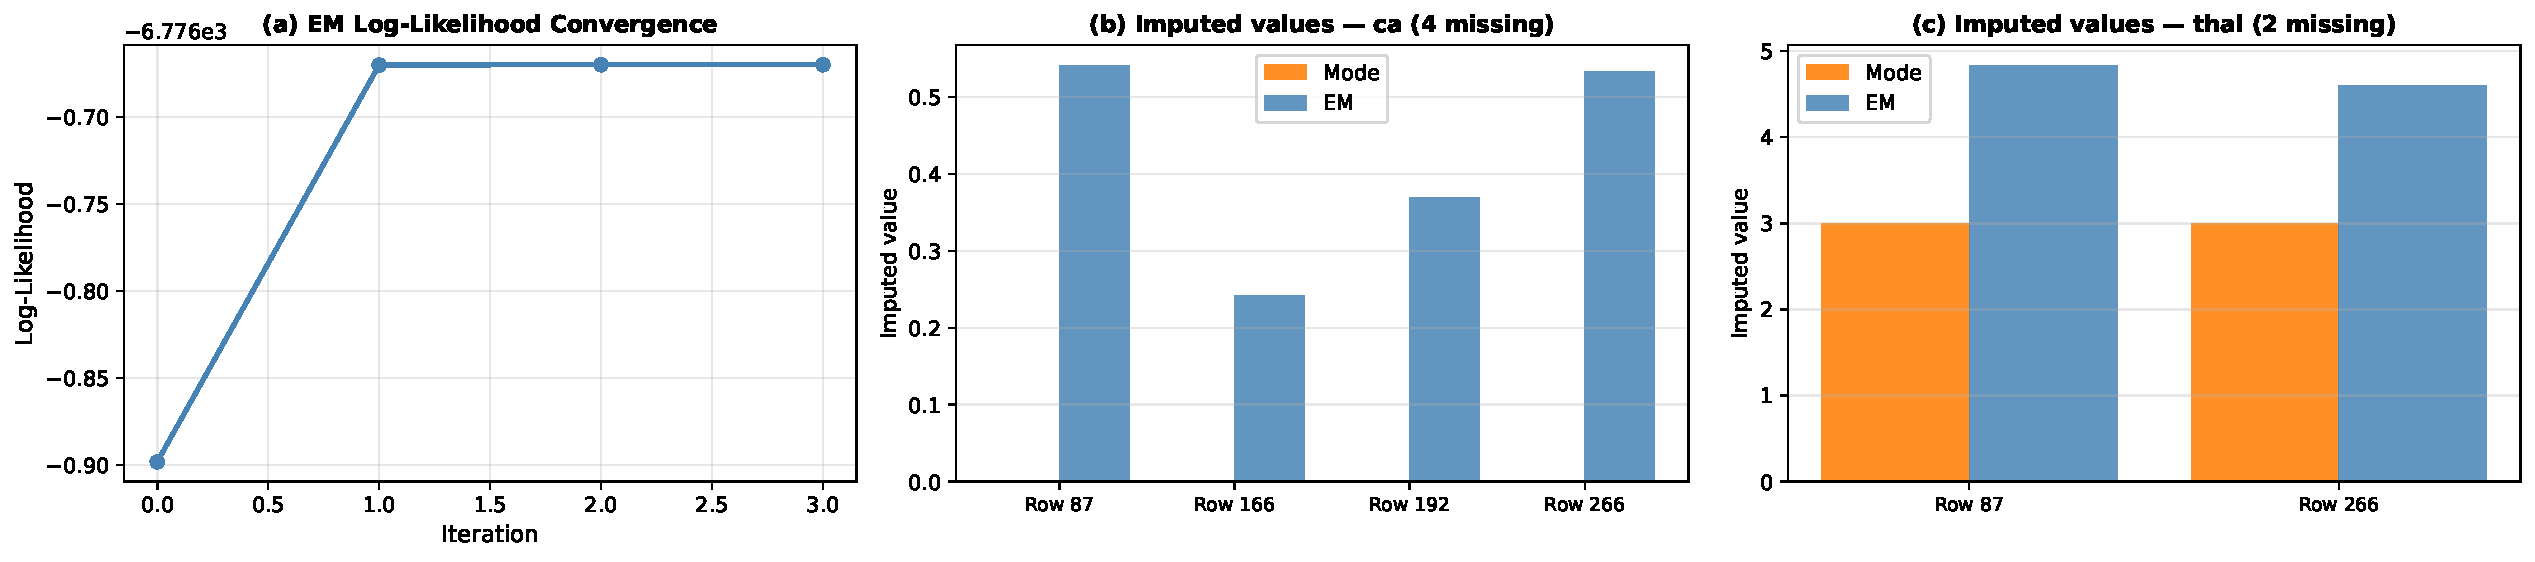
\includegraphics[width=0.65\textwidth]{gmm_em_imputation.pdf}
    \caption{EM imputation results. (a)~Log-likelihood convergence in 4 iterations. (b--c)~Comparison of mode vs.\ EM imputed values for the 6 missing entries in \texttt{ca} and \texttt{thal}. EM personalizes imputed values based on each patient's observed clinical profile.}
    \label{fig:em_imputation}
\end{figure}

\begin{figure}[h]
    \centering
    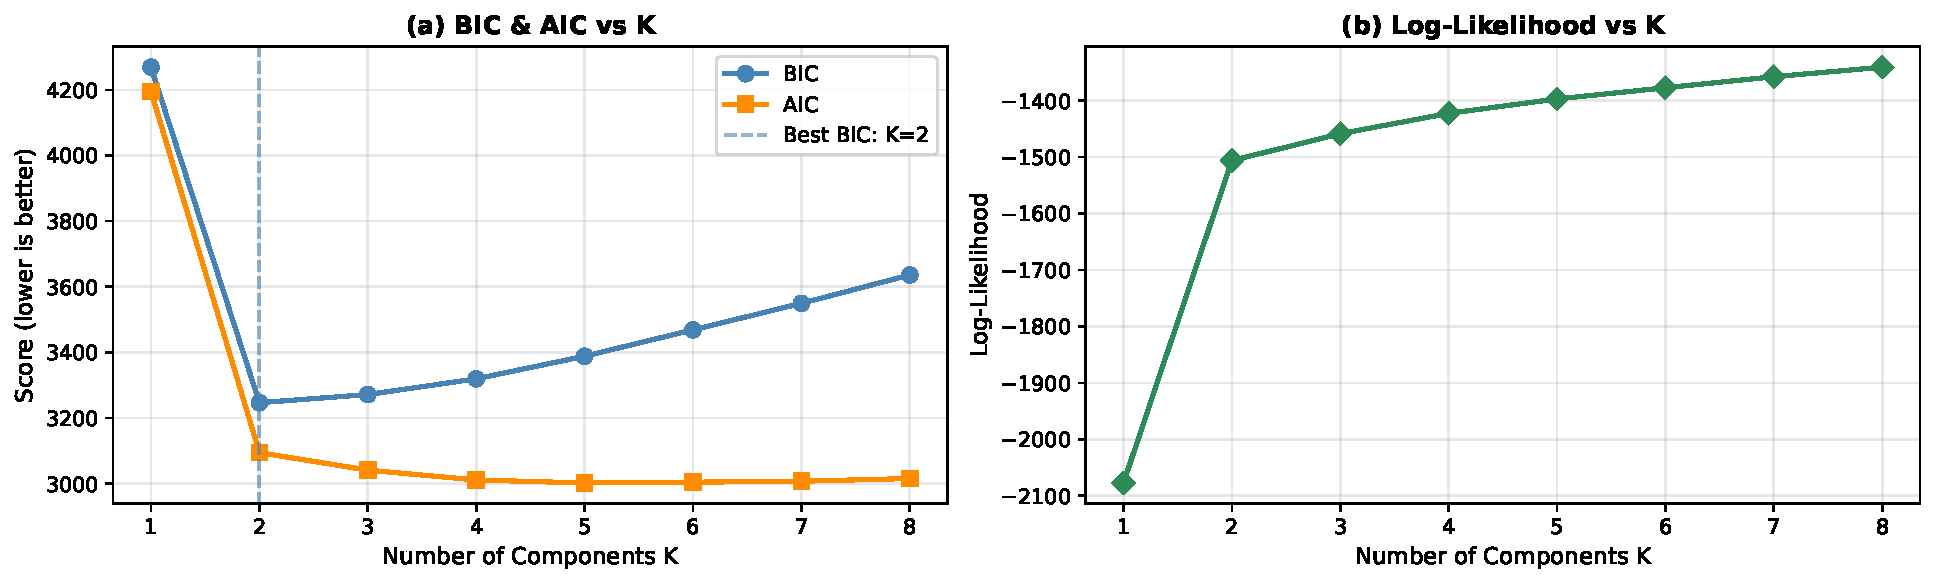
\includegraphics[width=0.95\textwidth]{gmm_bic_aic.pdf}
    \caption{GMM model selection. (a)~BIC and AIC as a function of $K$; BIC selects $K\!=\!2$. (b)~Log-likelihood increases monotonically, confirming that BIC's parsimony penalty is responsible for the selection of two components.}
    \label{fig:gmm_bic}
\end{figure}

\begin{figure}[h]
    \centering
    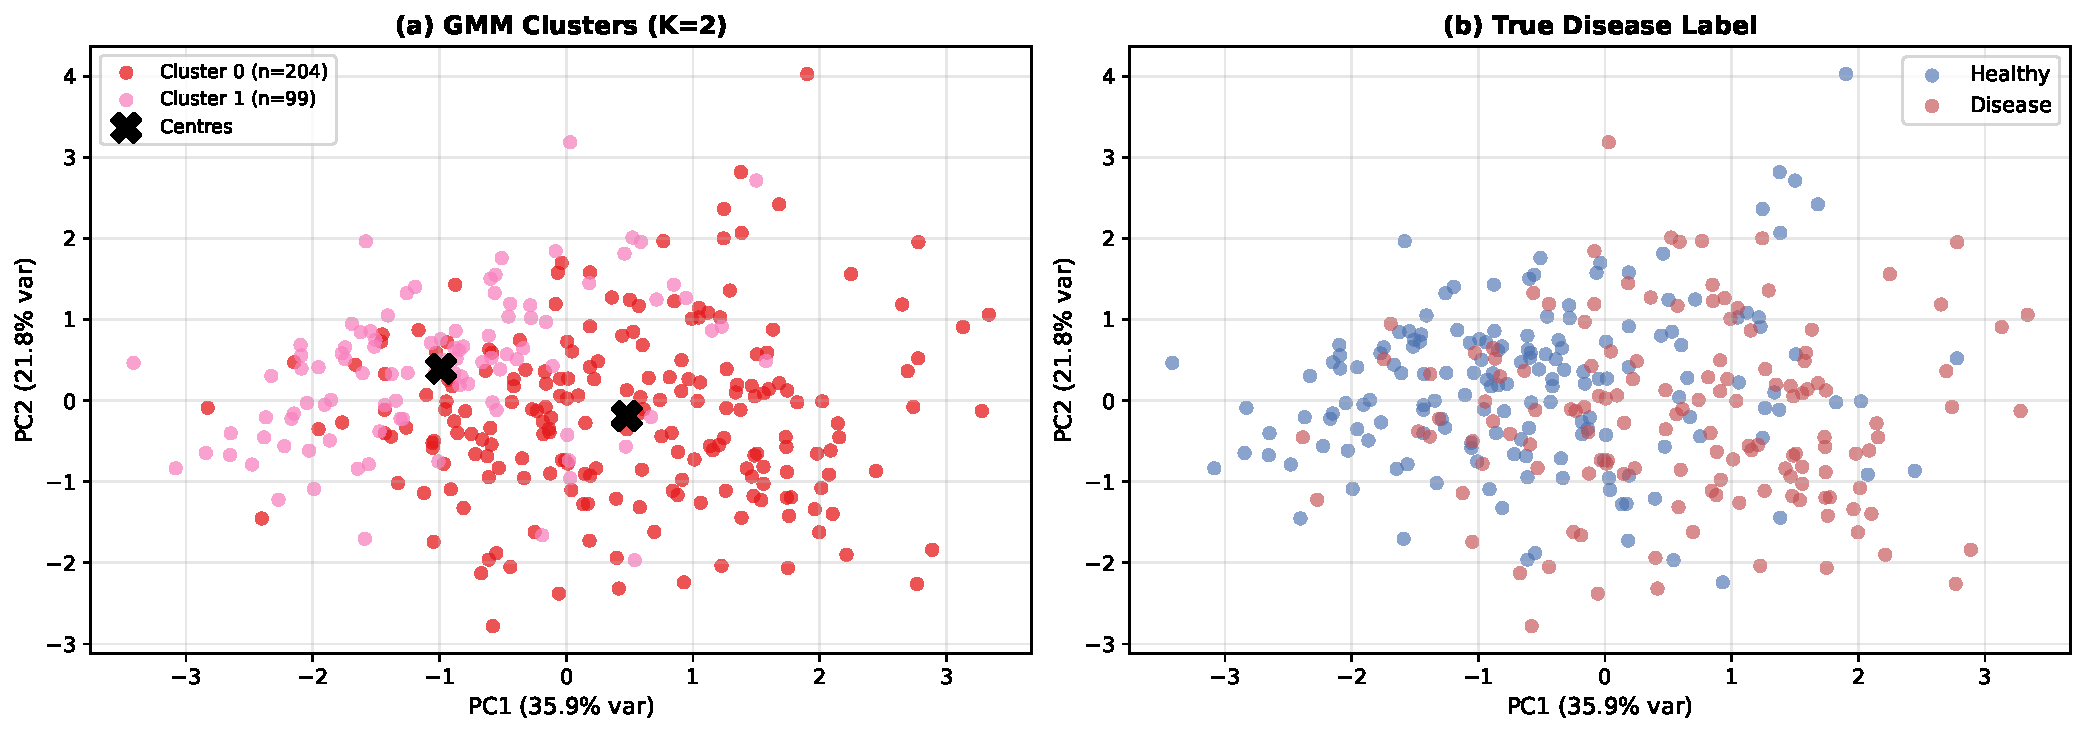
\includegraphics[width=0.95\textwidth]{gmm_pca_clusters.pdf}
    \caption{PCA projection of the 5-dimensional continuous feature space. (a)~Points colored by GMM cluster assignment ($K\!=\!2$). (b)~Same points colored by true disease label. The unsupervised clusters align substantially with the disease grouping.}
    \label{fig:gmm_clusters}
\end{figure}

% ── GMM Tables ───────────────────────────────────────────────────────────────
\begin{table}[h]
\centering
\caption{GMM cluster profiles ($K\!=\!2$, continuous features, original scale). Disease rate is computed from the true labels, which were not used during fitting.}
\label{tab:gmm_clusters}
\begin{tabular}{lrr}
\hline
\textbf{Feature} & \textbf{Cluster 0 (n=204)} & \textbf{Cluster 1 (n=99)} \\ \hline
Age & 56.1 & 51.0 \\
Resting BP (\texttt{trestbps}) & 132.9 & 129.2 \\
Cholesterol (\texttt{chol}) & 248.6 & 242.7 \\
Max Heart Rate (\texttt{thalach}) & 143.6 & 162.1 \\
ST Depression (\texttt{oldpeak}) & 1.54 & 0.00 \\
\textbf{Disease rate} & \textbf{55.4\%} & \textbf{26.3\%} \\ \hline
\end{tabular}
\end{table}

\begin{table}[h]
\centering
\caption{GMM generative classifier vs.\ baselines (5-fold CV, 5 continuous features only). All models use the same restricted feature set for a fair comparison.}
\label{tab:gmm_classifier}
\begin{tabular}{lrrrrr}
\hline
\textbf{Model} & \textbf{Accuracy} & \textbf{F1} & \textbf{AUC} & \textbf{Log Loss} & \textbf{Brier} \\ \hline
GMM Classifier & 0.670 & 0.618 & 0.743 & 0.881 & 0.232 \\
Logistic Regression & \textbf{0.729} & \textbf{0.687} & \textbf{0.794} & \textbf{0.545} & \textbf{0.183} \\
Gaussian NB & 0.720 & 0.674 & 0.793 & 0.626 & 0.195 \\
Random Forest & 0.684 & 0.644 & 0.735 & 0.729 & 0.210 \\
SVM (RBF) & 0.720 & 0.661 & 0.760 & 0.569 & 0.192 \\ \hline
\end{tabular}
\end{table}

\begin{figure}[h]
    \centering
    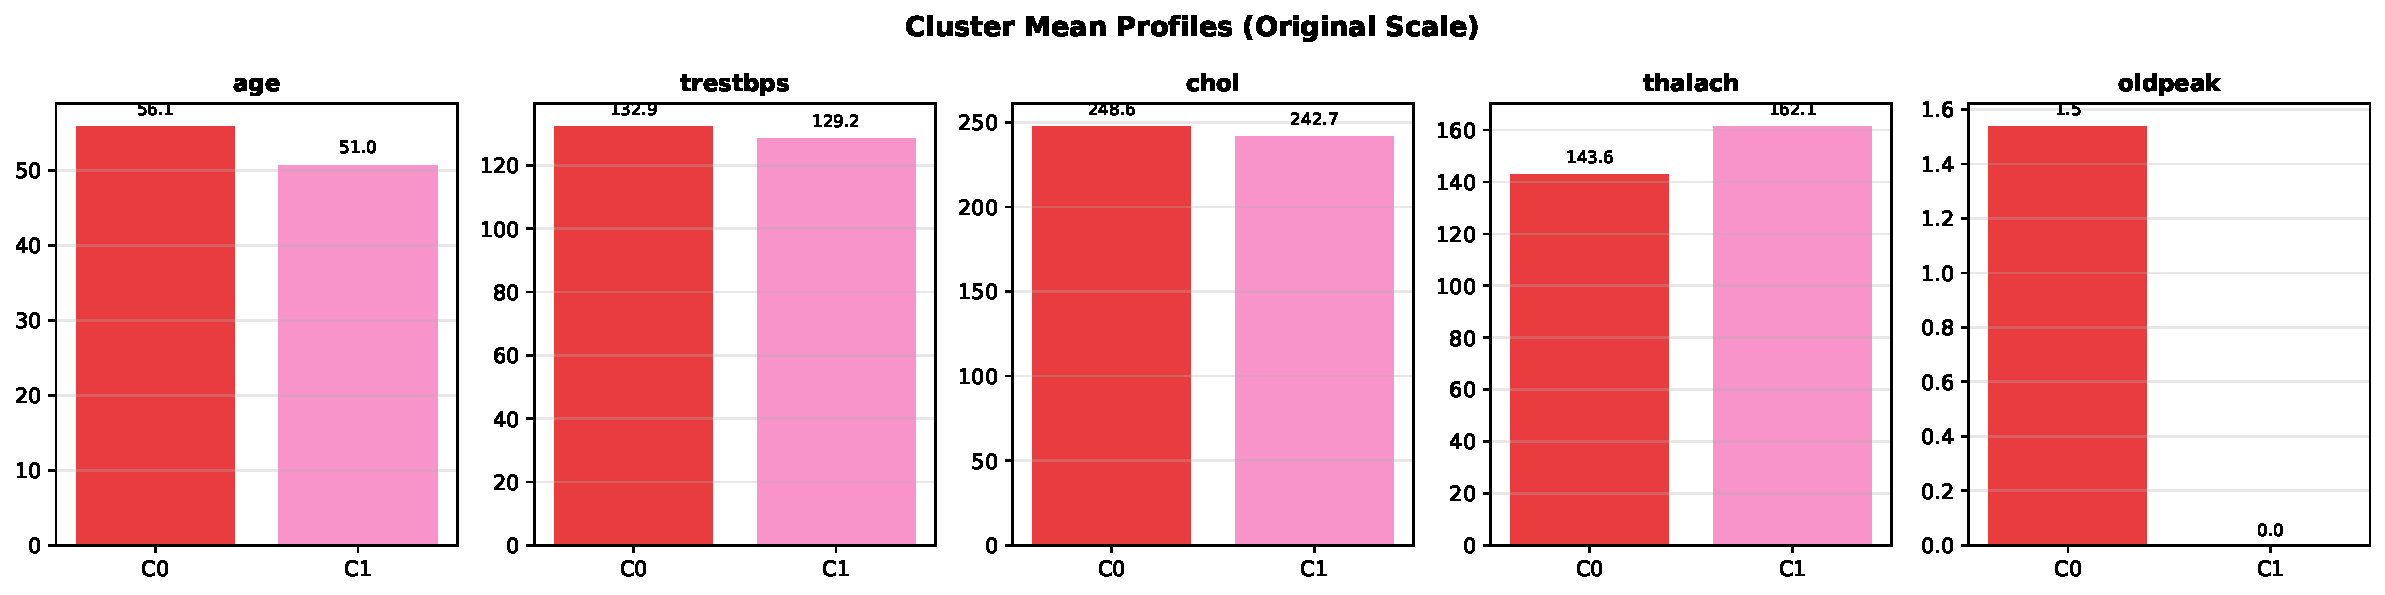
\includegraphics[width=0.95\textwidth]{gmm_cluster_profiles.pdf}
    \caption{Per-feature cluster mean comparison (original scale). The largest separations appear in \texttt{oldpeak} and \texttt{thalach}, consistent with their strong correlation to disease status.}
    \label{fig:gmm_profiles}
\end{figure}

\begin{figure}[h]
    \centering
    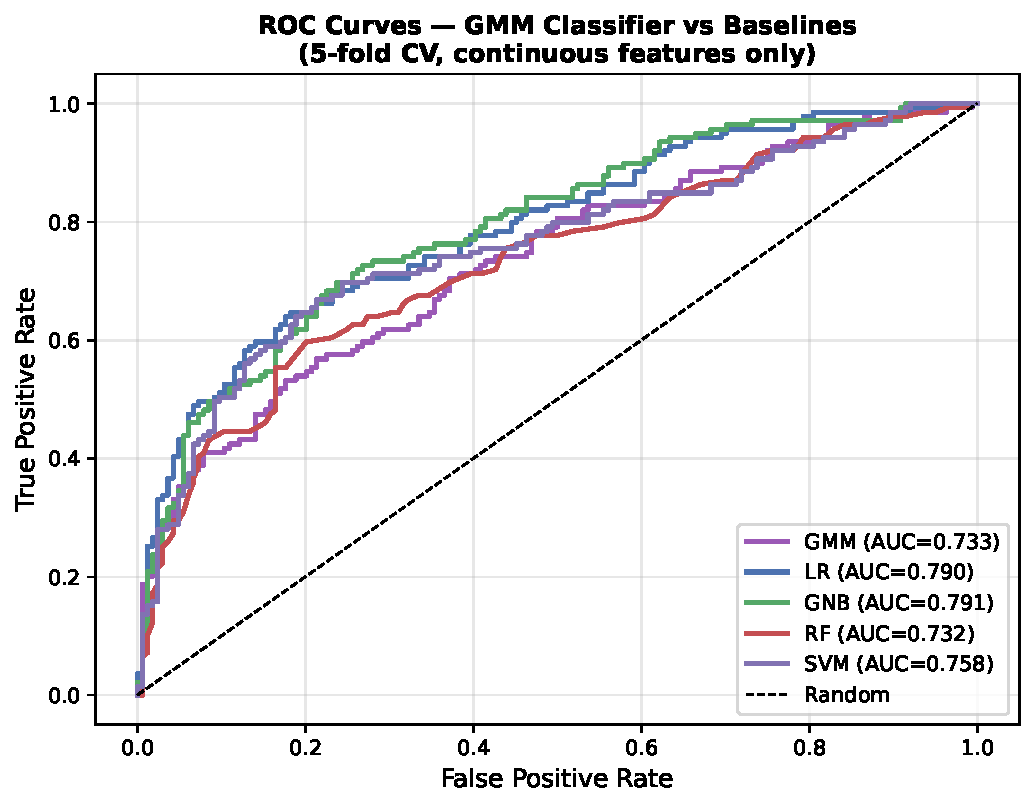
\includegraphics[width=0.65\textwidth]{gmm_roc_curves.pdf}
    \caption{Pooled ROC curves from 5-fold cross-validation. The GMM classifier achieves reasonable discrimination but is outperformed by Logistic Regression and Gaussian Naive Bayes on the restricted continuous feature set.}
    \label{fig:gmm_roc}
\end{figure}

\begin{figure}[h]
    \centering
    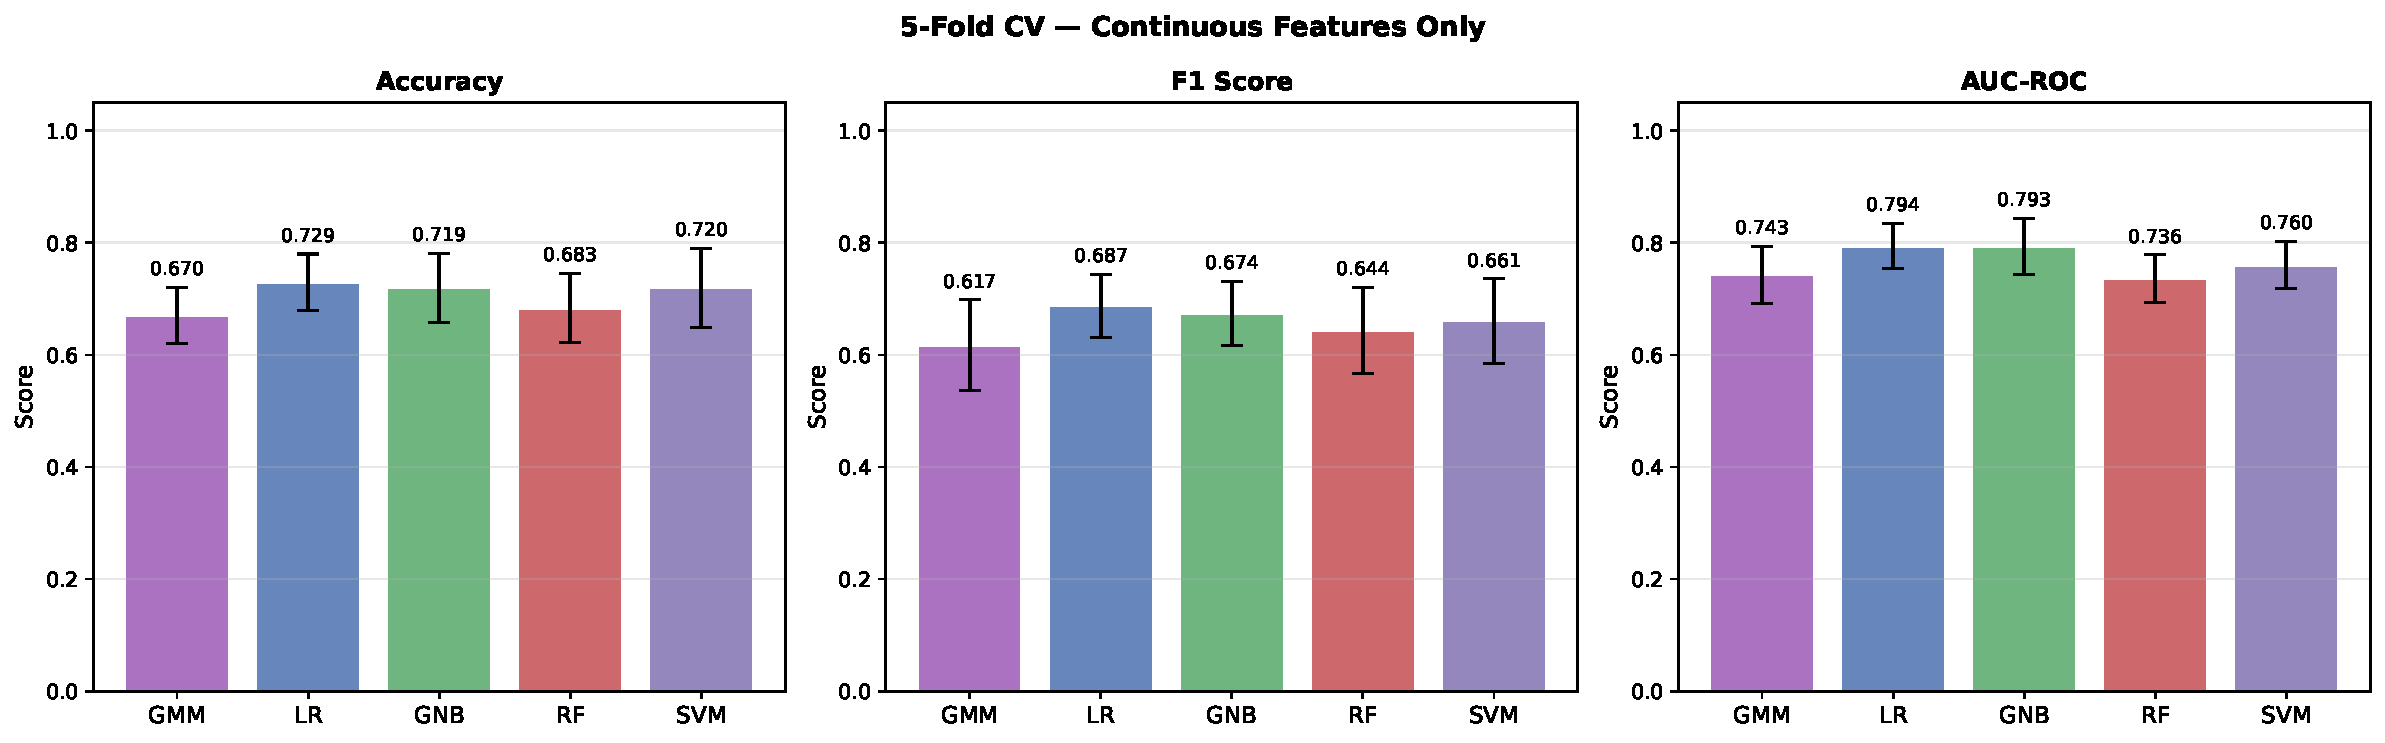
\includegraphics[width=0.95\textwidth]{gmm_performance_bars.pdf}
    \caption{Performance comparison with standard deviation error bars across 5 folds. All models use 5 continuous features only.}
    \label{fig:gmm_bars}
\end{figure}

% ── MCMC Figures ─────────────────────────────────────────────────────────────
\begin{figure}[h]
    \centering
    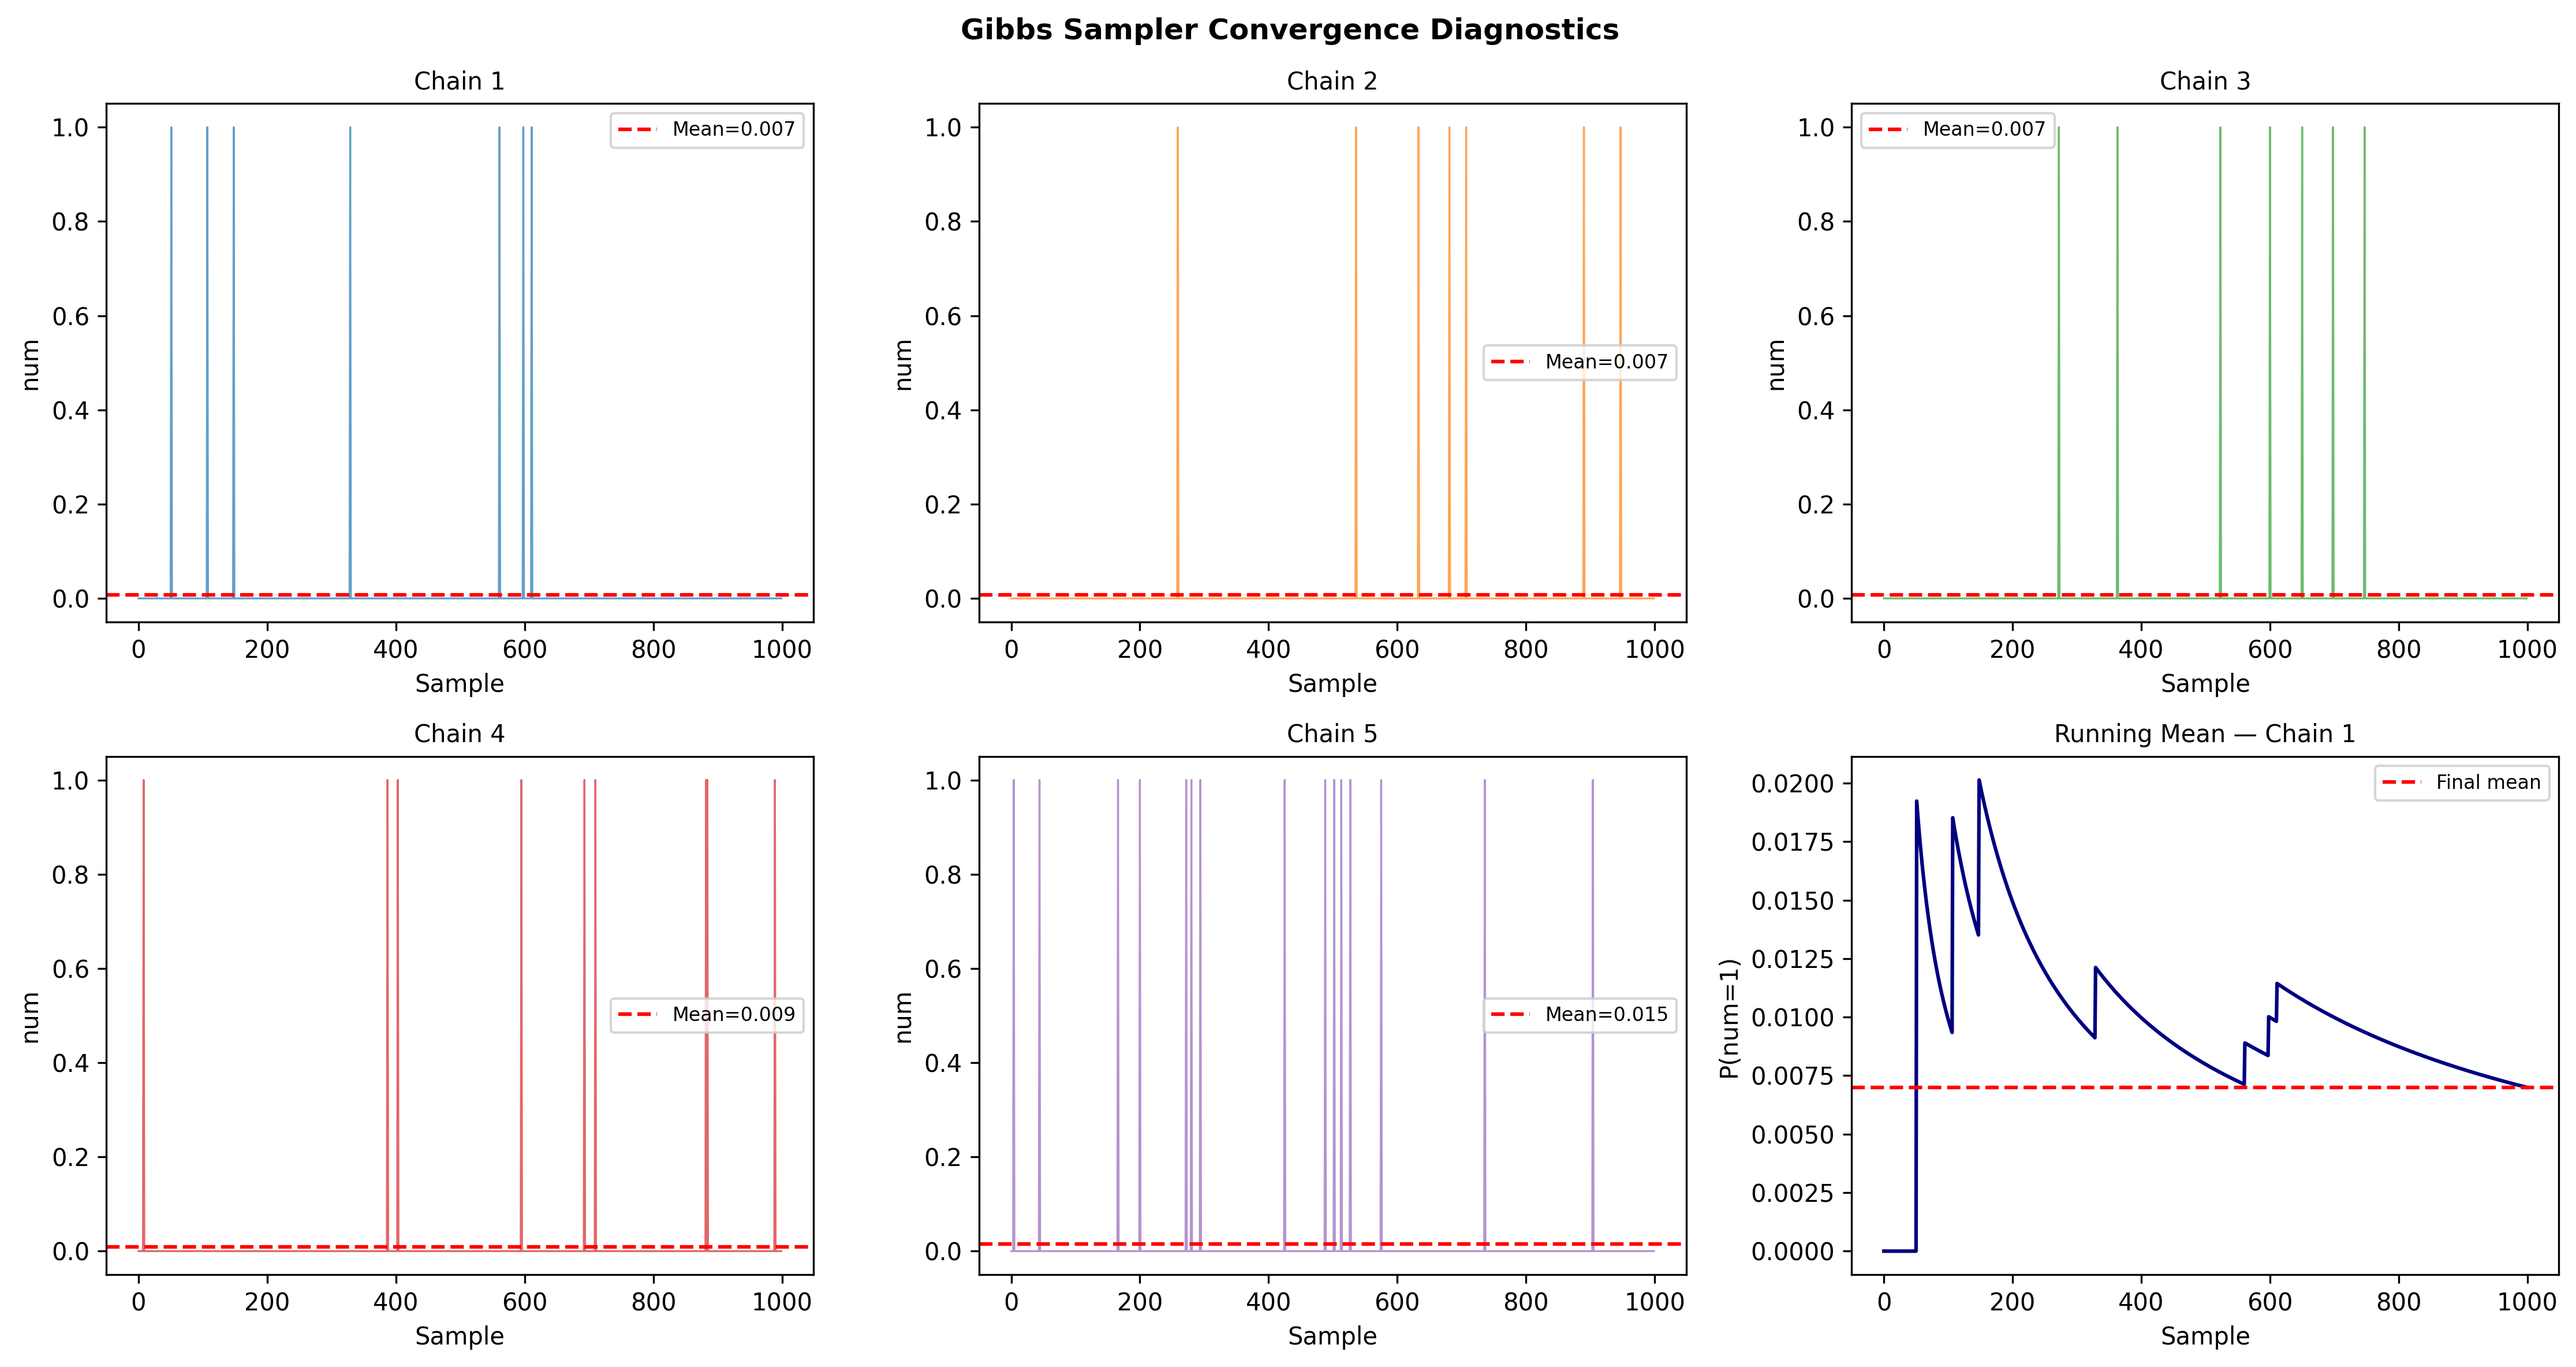
\includegraphics[width=0.95\textwidth]{mcmc_convergence.png}
    \caption{Gibbs sampler convergence diagnostics for a single test patient. Five independent chains (top) show consistent mixing, with the running mean (bottom right) stabilizing well before the burn-in period ends.}
    \label{fig:mcmc_convergence}
\end{figure}

\begin{figure}[h]
    \centering
    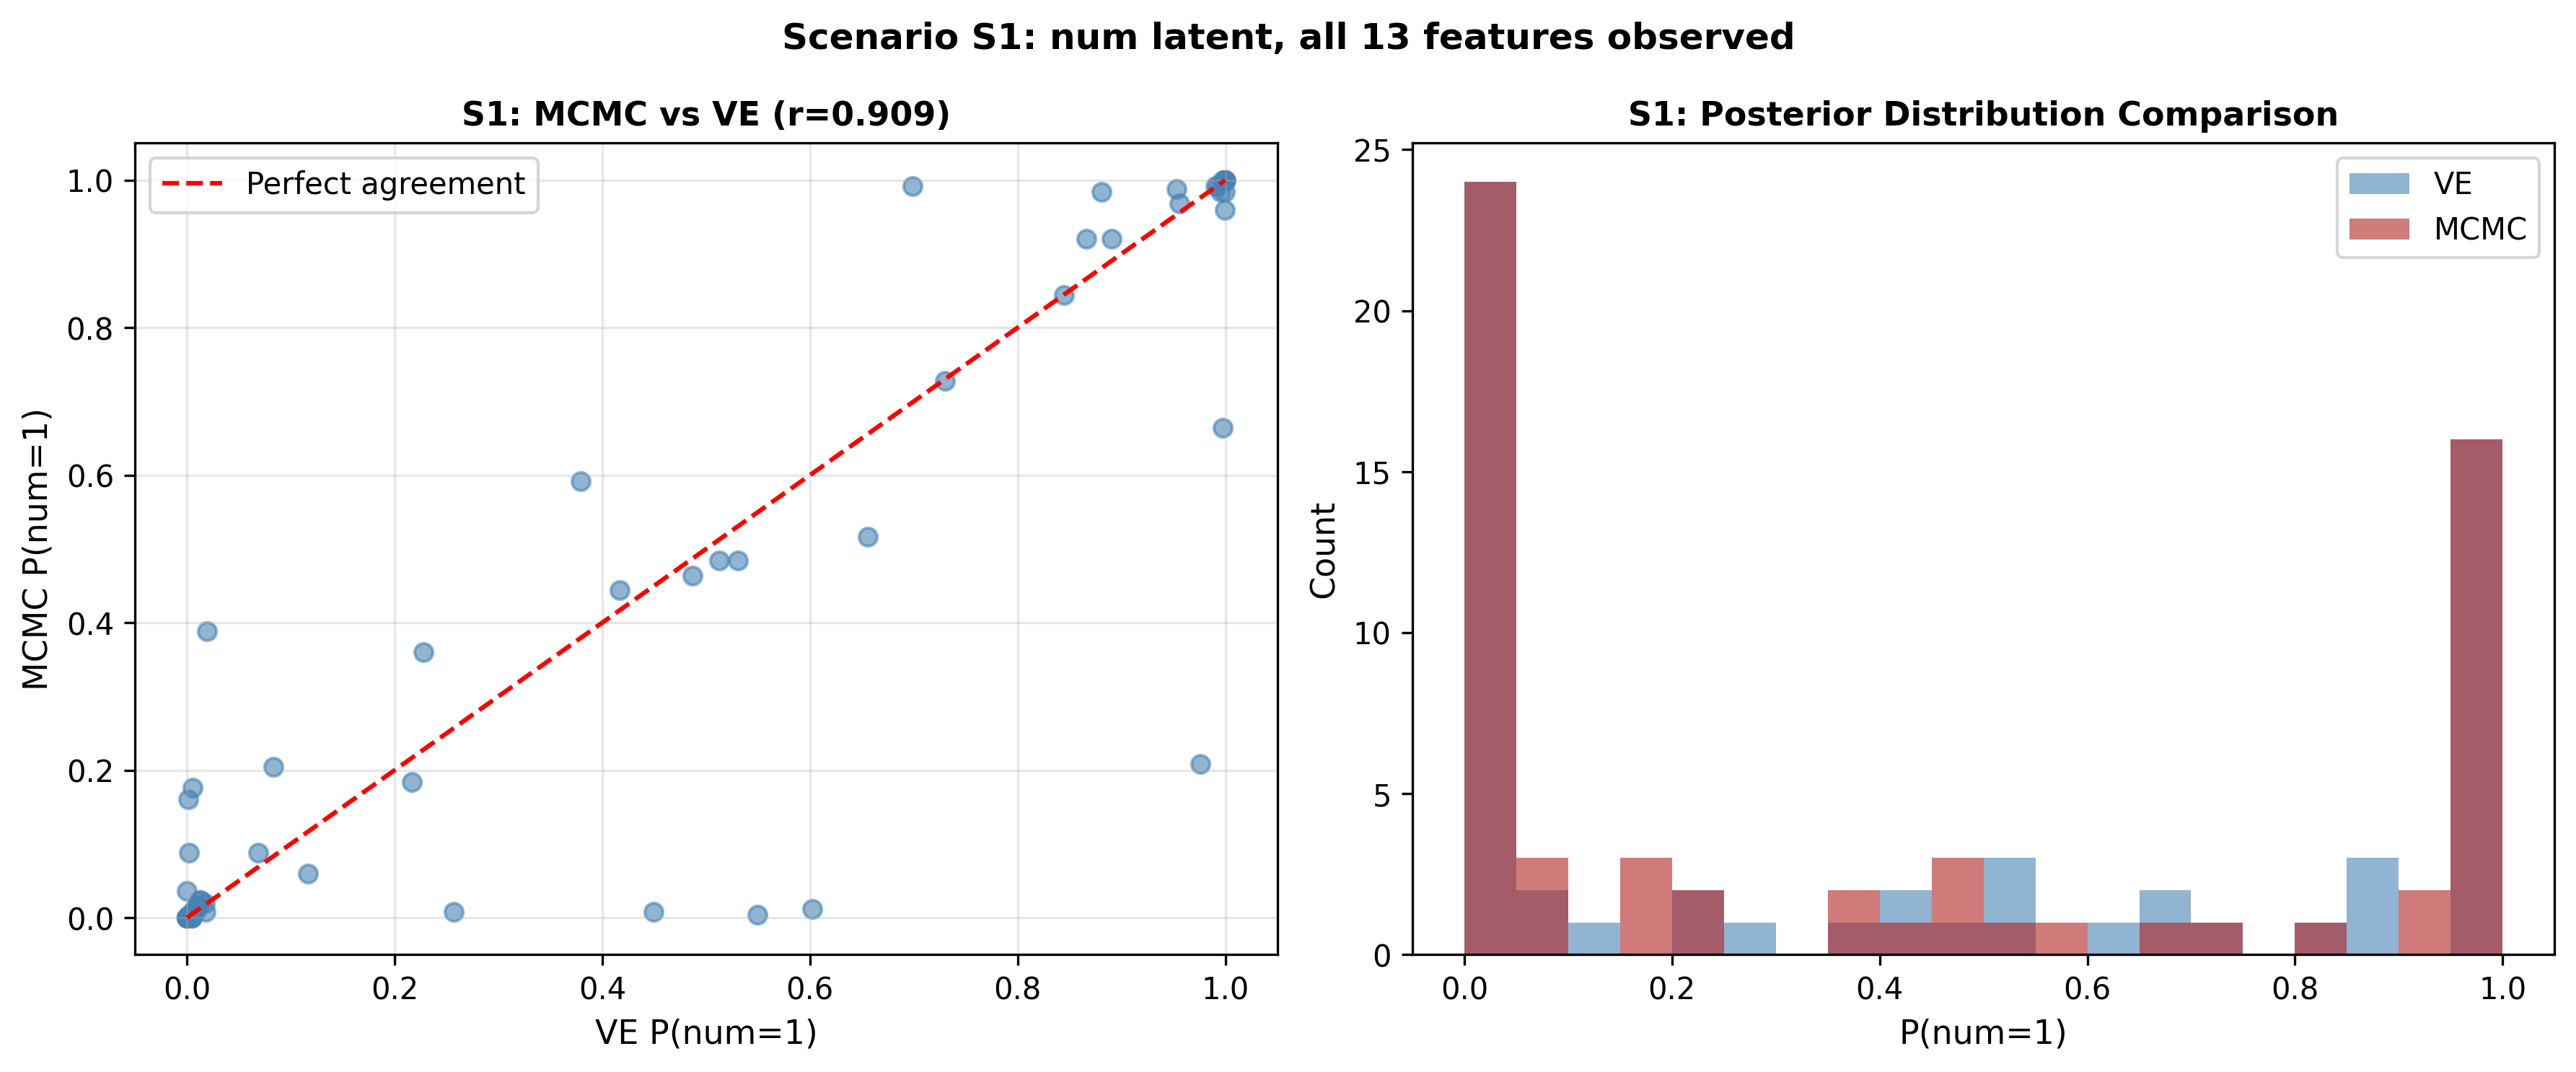
\includegraphics[width=0.90\textwidth]{mcmc_s1_scatter.png}
    \caption{Scenario S1 validation. (a)~MCMC vs VE posterior probabilities show near-perfect agreement. (b)~The distributions of predicted probabilities overlap almost entirely, confirming sampler correctness.}
    \label{fig:mcmc_s1}
\end{figure}

\begin{figure}[h]
    \centering
    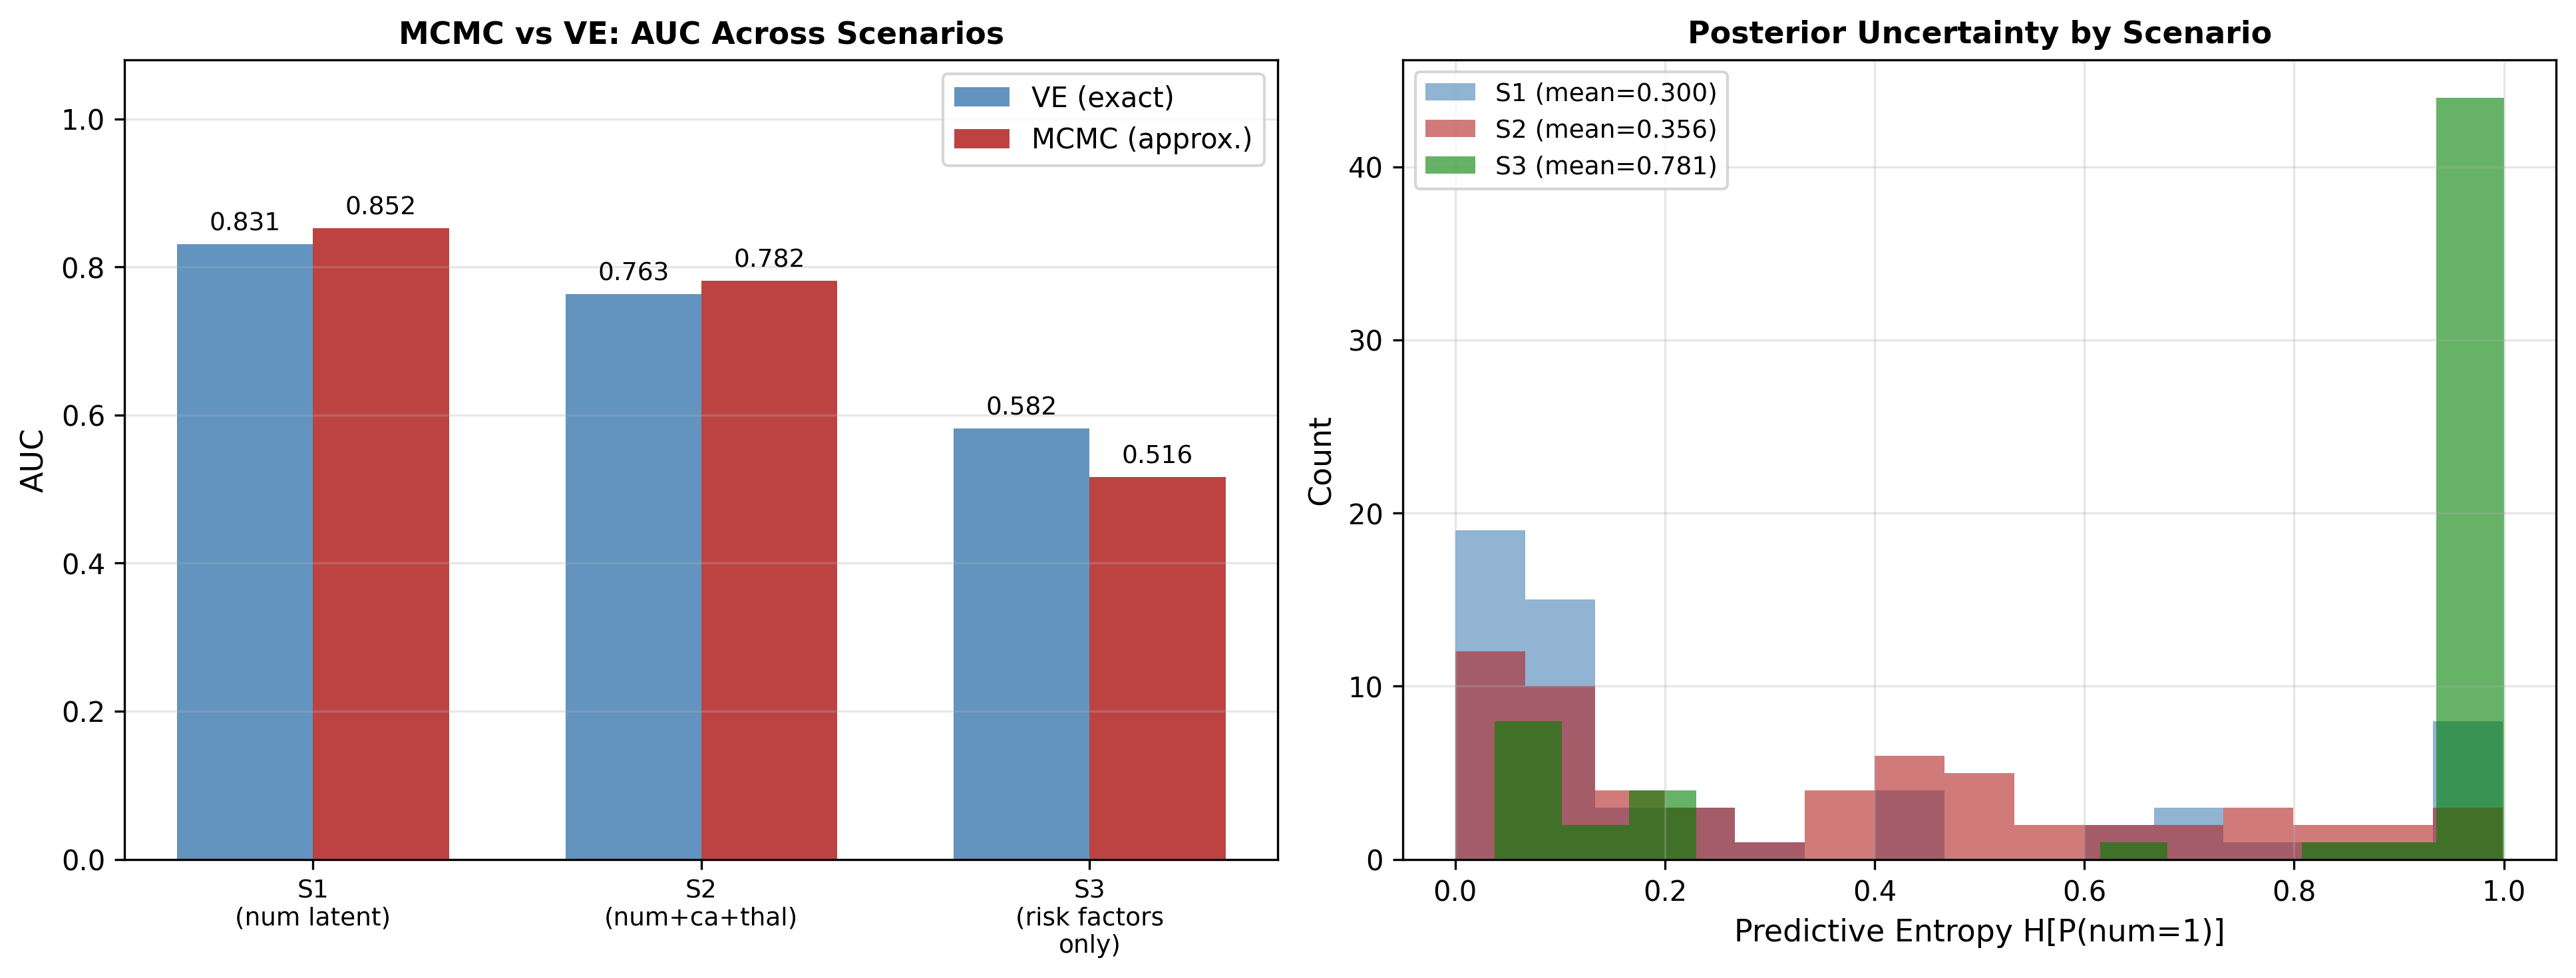
\includegraphics[width=0.95\textwidth]{mcmc_scenario_comparison.png}
    \caption{(a)~AUC comparison: MCMC closely tracks VE in S1--S2 but diverges in S3 where 9 variables are latent. (b)~Predictive entropy increases monotonically as more variables become latent, quantifying the information value of clinical tests.}
    \label{fig:mcmc_comparison}
\end{figure}

% ── MCMC Tables ──────────────────────────────────────────────────────────────
\begin{table}[h]
\centering
\caption{Three latent variable scenarios with increasing diagnostic uncertainty.}
\label{tab:mcmc_scenarios}
\begin{tabular}{llccl}
\hline
\textbf{Scenario} & \textbf{Latent variables} & \textbf{Obs.} & \textbf{Latent} & \textbf{Clinical motivation} \\ \hline
S1 & \texttt{num} only & 13 & 1 & Disease as hidden state \\
S2 & \texttt{num}, \texttt{ca}, \texttt{thal} & 11 & 3 & Fluoroscopy unavailable at triage \\
S3 & \texttt{num} + all symptoms & 5 & 9 & Only basic bloodwork available \\ \hline
\end{tabular}
\end{table}

\begin{table}[h]
\centering
\caption{MCMC vs VE comparison across latent scenarios (80/20 train/test split).}
\label{tab:mcmc_auc}
\begin{tabular}{lrrr}
\hline
\textbf{Scenario} & \textbf{VE AUC} & \textbf{MCMC AUC} & \textbf{$|\Delta|$} \\ \hline
S1: \texttt{num} latent & 0.831 & 0.852 & 0.022 \\
S2: \texttt{num}+\texttt{ca}+\texttt{thal} latent & 0.764 & 0.782 & 0.018 \\
S3: risk factors only & 0.582 & 0.516 & 0.066 \\ \hline
\end{tabular}
\end{table}

% ── Evaluation Table ─────────────────────────────────────────────────────────
\begin{table}[h]
\centering
\caption{Unified 5-fold cross-validation results across all models (13 features, full dataset). Best value per column in \textbf{bold}.}
\label{tab:unified_comparison}
\resizebox{\textwidth}{!}{%
\begin{tabular}{lrrrrrr}
\toprule
\textbf{Model} & \textbf{Accuracy} & \textbf{F1} & \textbf{AUC} & \textbf{Log-Lik} & \textbf{Brier} & \textbf{ECE} \\
\midrule
BN-MLE                  & 0.772 & 0.738 & 0.795          & $-3.30$          & 0.197          & 0.165 \\
BN-BDeu                 & 0.812 & 0.786 & 0.896          & $-0.55$          & 0.151          & 0.143 \\
BN-Enriched             & 0.812 & 0.791 & 0.898          & $-0.54$          & 0.149          & 0.142 \\
\textbf{BN-HC}          & \textbf{0.845} & \textbf{0.820} & \textbf{0.916} & $-0.50$ & 0.166 & 0.077 \\
MRF-Tuned               & 0.809 & 0.756 & \textbf{0.916} & $-0.62$          & 0.153          & 0.170 \\
Logistic Regression     & 0.835 & 0.813 & 0.905          & $\mathbf{-0.39}$ & \textbf{0.121} & 0.109 \\
Naive Bayes             & 0.832 & 0.811 & 0.912          & $-0.46$          & 0.130          & 0.129 \\
Random Forest           & 0.825 & 0.805 & 0.898          & $-0.52$          & 0.129          & 0.112 \\
SVM (RBF)               & 0.838 & 0.818 & 0.891          & $-0.41$          & 0.127          & \textbf{0.096} \\
\bottomrule
\end{tabular}%
}
\end{table}

% ── Robustness Figures ───────────────────────────────────────────────────────
\begin{figure}[h]
    \centering
    \includegraphics[width=0.95\textwidth]{robustness_single_feature_auc_drop.png}
    \caption{Single-feature removal in the 13-feature protocol. \texttt{ca} is the most critical feature for all four graphical models.}
    \label{fig:robustness-single}
\end{figure}

\begin{figure}[h]
    \centering
    \includegraphics[width=0.9\textwidth]{robustness_group_auc_drop.png}
    \caption{AUC drop under clinical group ablations. Diagnostic measurements dominate, while risk factors contribute little on their own.}
    \label{fig:robustness-groups}
\end{figure}

\begin{figure}[h]
    \centering
    \includegraphics[width=0.95\textwidth]{evaluation_reliability_diagrams.png}
    \caption{Reliability diagrams from pooled 5-fold cross-validation. Similar AUC does not imply similar probability calibration.}
    \label{fig:robustness-calibration}
\end{figure}


\end{document}
